\documentclass[../../InformazioneQuantistica.tex]{subfiles}

\begin{document}

\section{Crittografia e meccanica quantistica}
\lesson{9 \orangedot}{27/3/2019}
Con \textbf{crittografia}\index{Crittografia} si intende l'insieme di tecniche necessarie a rendere una comunicazione \textit{sicura}, ossia inaccessibile a chiunque non sia il destinatario inteso.\\ 
Nel corso della storia si sono susseguiti metodi via via più sofisticati per ottener ciò. Per esempio, i romani utilizzavano una striscia di cuoio da attorcigliare attorno ad un'asta di legno. Il messaggio confidenziale era quindi scritto \textit{in verticale} sul nastro, che poi veniva srotolato, risultando così in una sequenza disordinata di caratteri. In questo modo, solo disponendo di un bastone con lo stesso diametro era possibile replicare la configurazione iniziale, e quindi leggere il messaggio. Tale asta è quindi detta \textbf{chiave} (e in questo caso è proprio un oggetto fisico), in quanto consente a chi la possiede di \textit{accedere} al contenuto del messaggio cifrato senza difficoltà.\\
In crittografia si suppone che la \textit{chiave} sia condivisa tra mittente e destinatario, e che nessun altro ne sia in possesso. Il meccanismo di cifratura, tuttavia, può essere di dominio pubblico: un cifrario si dice \textit{sicuro} se, pur conoscendone perfettamente il meccanismo, non è possibile decifrarne i messaggi senza conoscere la chiave.\\

Parallelamente alla crittografia, la \textbf{crittoanalisi} si occupa di \q{forzare} i cifrari, ossia svelarne i contenuti cifrati senza essere in possesso delle informazioni necessarie per farlo (ossia della chiave).\\

Per esempio, un \textit{cifrario} molto comune in passato è la cosiddetta \textbf{sostituzione monoalfabetica}, che consiste nel sostituire ogni carattere del messaggio con un altro. La chiave è allora data da una tabella che mostra le sostituzioni effettuate, permettendo quindi di invertirle e decifrare il messaggio.\\
In ogni lingua, tuttavia, certe lettere compaiono più frequentemente di altre. Da un'analisi statistica delle frequenze del messaggio cifrato (che supponiamo sufficientemente lungo) è perciò possibile riconoscere una certa parte delle sostituzioni, e ricavare \textit{per tentativi} le altre - ricostruendo così la chiave. Perciò la \textit{sostituzione monoalfabetica} non è, al giorno d'oggi, un cifrario sicuro.

\subsection{Crittografia classica}
Possiamo schematizzare il processo crittografico come una \textbf{trasformazione}\marginpar{Definizione di cifrario} $\hat{E}_K$ (\textit{encryption}) che mappa il messaggio da cifrare $P$ (\textit{plaintext}) nel messaggio cifrato $C$ (\textit{ciphertext}), e che dipende da un parametro $K$ detto chiave (\textit{key}):
\begin{align*}
P \mapsto \hat{E}_K(P) = C
\end{align*}
 Tale trasformazione deve essere invertibile: possedendo $K$ si può decifrare $C$ e riottenere $P$. Esiste quindi una mappa inversa $\hat{D}_K$ (\textit{decryption}):
\begin{align*}
C \mapsto \hat{D}_K(C) = P
\end{align*}

Consideriamo uno schema specifico per $\hat{E}_K$ (\textbf{cifrario di Vernam})\marginpar{Cifrario di Vernam}. Partiamo associando ad ogni lettera un codice numerico:
\begin{align*}
A\mapsto 00, \> B \mapsto 01, \> C \mapsto 02, \dots , Z \mapsto 26
\end{align*}
Possiamo allora prendere un messaggio $P$=\q{Shaken not stirred}, e una chiave $K$ composta di numeri casuali, e combinarle \textit{un numero alla volta} per formare il messaggrio criptato $C$:
\begin{align*}
\hat{E}_K(P_i) = (P_i + K_i)_{\op{mod}26} = C_i
\end{align*}
La trasformazione inversa è data da:
\begin{align*}
\hat{D}_K(C_i) = (C_i - K_i)_{\op{mod}26} = P_i
\end{align*}

\begin{expl}
Tale schema può essere implementato facilmente in un computer convertendo $P$ e $K$ in una serie di \textit{bit} (per esempio tramite il codice ASCII). Detti allora $\{p_1, p_2, \dots, p_N\}$ i bit del messaggio e $\{k_1, \dots, k_N\}$ quelli della chiave (con $k_i \in \{0,1\}$ e $p_i \in \{0,1\}$) si ha:
\begin{align*}
c_i = \hat{E}_{K}(p_i) = p_i \oplus k_i \quad \forall i = 1, 2, \dots, N
\end{align*}
dove $\oplus$ indica uno XOR, che equivale ad una somma in modulo $2$. Per decifrare lo schema è il medesimo:
\begin{align*}
p_i = \hat{D}_K(c_i) = c_i \oplus k_i \quad \forall i =1, 2, \dots, N
\end{align*}
\end{expl}
Matematicamente, si dimostra che tale processo genera messaggi sicuri, nel senso di \textit{completamente indecifrabili}, solo se $K$ ha le seguenti proprietà:
\begin{itemize}
\item $K$ è completamente casuale
\item $K$ è usata una volta sola (\textit{One Time Pad})
\end{itemize}

\begin{expl}
\textbf{Sicurezza del cifrario di Vernam}. Se la chiave $K$ è casuale ed è \textit{lunga quanto il messaggio} $P$, anche il messaggio cifrato $C$ sarà, effettivamente, composto di caratteri \textit{casuali}. Procedendo per \textit{forza bruta}, tentando tutte le chiavi $K$ possibili, è possibile decifrare da $C$ una qualsiasi stringa di testo: il messaggio cercato è perciò \textit{nascosto} tra una miriade di \q{messaggi spurii} che, non conoscendo $K$, risultano ugualmente validi. Per esempio, il messaggio originale potrebbe essere il seguente:
\begin{align*}
\underset{\texttt{\normalsize\hspace{-5pt}C: \textcolor{Red}{Ab flf bdks bh xas xrar B dmhz gfqqkn mbh}}}{\underset{\texttt{\normalsize \hspace{-5pt}K: So meb odyo nc eto ldme t hewo rldisg onn}}{\texttt{P: In the name of the moon I will punish you!}}}
\end{align*}
Una scelta casuale di $K$ può produrre però $P$ completamente diversi, ma lo stesso \q{sensati}:
\begin{align*}
\underset{\texttt{\normalsize\hspace{-0pt}P: Hey you youre finally awake You were tr}}{\underset{\texttt{\normalsize \hspace{-0pt}K: Txh nrh fwykd ssfxgpt Bhmxv irw ugwi iq}}{\texttt{C: 
\textcolor{Red}{Abf lfb dksbh xasxrar bdmhz Gfq qknm bh}}}}
\end{align*}
Se la chiave $K$ è scelta casualmente\footnote{Quindi non come nell'esempio appena visto...} non vi sono scelte \q{più probabili} di altre, e quindi non vi è alcun modo per ricavare il messaggio $P$ corretto, e nemmeno quelli \q{più probabili}.\\

Risulta però di estrema importanza \textbf{non riutilizzare} la stessa chiave $K$. In tal caso, infatti, è possibile immediatamente ricavare informazioni sui messaggi cifrati. Siano $a_i$ e $b_i$ i caratteri di due messaggi (con alfabeto di $N$ caratteri), e $k_i$ quelli della chiave usata per cifrare entrambi. Si ha allora:
\begin{align*}
c_i = a_i + k_i \mod N; \quad d_i = b_i + k_i \mod N
\end{align*}
Sottraendo membro a membro:
\begin{align}
c_i - d_i \mod N = a_i + k_i -b_i -k_i \mod N = a_i-b_i \mod N
\label{eqn:a-b}
\end{align}
Si trova così una relazione diretta tra i due messaggi. Si può ora procedere \textit{per tentativi}, cercando di indovinare singole parole di $A$ e $B$ compatibili con tale relazione, in un processo detto \textit{crib drag}. L'idea di base è che vi sono parole comuni  facilmente  contenute in ogni messaggio (es. \textit{the} in inglese). Per esempio, ipotizzando che $\{b_{i}\}_{i=1,\dots,5} = \text{\q{Hello}}$, possiamo ricavare da (\ref{eqn:a-b}) le prime $5$ lettere di $A$. Se queste ultime \q{hanno senso} (per esempio risultano in \q{Helpm}) allora si ha conferma del tentativo appena fatto. Possiamo ora \textit{espandere} quanto ricavato per $A$ (es. \q{Help me please}) e di conseguenza ottenere nuovi caratteri di $B$, che - ammesso abbiano senso - possono portare a loro volta a nuove ipotesi, e così via.\\
Poiché un computer può tentare migliaia di parole comuni in ogni possibile posizione dei messaggi $A$ e $B$, la ripetizione di una chiave vanifica la sicurezza del cifrario di Vernam.
\end{expl}

La sicurezza del cifrario di Vernam richiede quindi di poter condividere una chiave $K$ che ha la stessa lunghezza del testo, e che deve pervenire unicamente al destinatario. Si presuppone quindi di avere un canale sicuro per fare questo passaggio: peccato che questo fosse proprio il problema che volevamo risolvere in partenza!\\
Un tale schema, detto \textbf{a cifratura simmetrica}, pone quindi il problema della \textbf{distribuzione delle chiavi}, che non è di facile risoluzione. Lo scenario peggiore si ha se qualcuno riesce a \textit{intercettare} la chiave senza che né mittente né destinatario se ne accorgano, poiché in tal caso il canale ritenuto sicuro è invece compromesso.

\subsection{Quantum Key Distribution (QKD)}
\marginpar{\danger Parte non ancora ricontrollata}
Tecniche di Informazione Quantistica permettono di risolvere il problema di distribuzione delle chiavi. Vi sono protocolli principali per farlo:
\begin{itemize}
\item \textbf{BB84}, che fa uso del principio di sovrapposizione e del no-cloning theorem
\item \textbf{E91}, per cui invece si usa l'entanglement
\end{itemize}

\subsection{Il protocollo BB84}
Supponiamo che \textbf{Alice} (A) voglia trasmettere a \textbf{Bob} (B) una chiave da utilizzare per future comunicazioni crittografate, facendo sì che nessuno possa intercettarla.\\

Alice può generare qubit nelle basi $B_z$ (autoket di $\hat{\sigma}_x$) o $B_x$ (autoket di $\hat{\sigma}_y$). Nella base computazionale $\{\ket{0}, \ket{1}\}$ possiamo esprimerli così:
\begin{align*}
B_z = \{\ket{0}, \ket{1}\} \qquad B_x =\{ \frac{1}{\sqrt{2}}(\ket{0}+\ket{1}), \frac{1}{\sqrt{2}}(\ket{0}-\ket{1})\}
\end{align*}

Il protocollo prosegue perciò nel seguente modo:
\begin{enumerate}
\item Alice genera una stringa di \textit{bit classici} completamente casuali:
\begin{align*}
K_1=0011100000001101
\end{align*}
\item Alice codifica la stringa $K_1$ associando ad ogni $0$ un qubit nello stato $\ket{0}$ o $\ket{+}$ in modo equiprobabile (metà degli $0$ diverranno $\ket{0}$, metà diverranno $\ket{+}$). Fa lo stesso per gli $1$, codificandoli o con $\ket{1}$ o con $\ket{-}$. Ottiene quindi una sequenza di qubit $K_2$:
\begin{align*}
K_2 =\ket{0},\ket{+},\ket{1}\ket{1}\ket{-}\ket{0}\ket{+}\ket{+}\dots
\end{align*}
\item Alice trasmette $K_2$ a Bob mediante un canale quantistico
\item Bob misura ciascun qubit nella base $B_x$ o $B_z$ in modo casuale, e registra i risultati in una stringa di bit classici $K_3$. Avremo allora due possibilità:
\begin{itemize}
\item Se Bob sceglie di misurare un qubit nella stessa base che Alice aveva usato per inviarlo, allora riottiene lo stesso bit classico che era stato usato in partenza
\item Se invece Bob usa una base diversa da Alice otterrà un risultato \textit{casuale}.
\end{itemize}
Per esempio, se Bob sceglie di misurare con $B_z, B_x, B_z, B_x, \dots$ potrebbe ottenere per $K_3$:
\begin{align*}
K_3 = 001010\dots
\end{align*}
\item A questo punto Alice e Bob condividono le \textbf{basi} utilizzate rispettivamente per generare o misurare gli stati dei qubit:
\begin{align*}
\text{Alice}: &\hlc{Yellow}{B_z}, \hlc{Yellow}{B_x}, \hlc{Yellow}{B_z}, B_z, \hlc{Yellow}{B_x}, B_z, B_x, \hlc{Yellow}{B_x}\\
\text{Bob}: &\hlc{Yellow}{B_z}, \hlc{Yellow}{B_x}, \hlc{Yellow}{B_z}, B_x, \hlc{Yellow}{B_x}, B_x, B_z, \hlc{Yellow}{B_x}
\end{align*}
A questo punto Alice e Bob sanno in quali casi il bit classico è sicuramente pervenuto all'altro. Basta allora tenere tali bit \q{sufficientemente inviati} e comporre con essi la chiave:
\begin{align*}
K =00100\dots
\end{align*}
\end{enumerate}

\begin{figure}[H]
\centering
\includegraphics[width=0.8\textwidth]{Immagini/27_3/image005.png}
\caption{Esempio di distribuzione quantistica di una chiave tramite il protocollo BB84. Alice parte da una sequenza di bit iniziale e la converte in una successione di qubit in $4$ stati possibili. Solo quando Bob misura il qubit nella stessa base usata da Alice per generare gli stati allora il bit classico iniziale è stato correttamente ricevuto.\label{fig:quantum-bb84}}
\end{figure}

Immaginiamo che una terza persona, \textbf{Eve}, cerchi di intercettare il messaggio. Per farlo \textbf{non può} duplicarlo (no-cloning theorem), e quindi l'unico modo è fare direttamente delle misure, secondo una sequenza di basi nuovamente arbitraria. Poiché è molto difficile che Eve faccia al $100\%$ le stesse scelte di Bob, quando A e B si scambiano le informazioni sulle basi utilizzate, Eve potrà al più recuperare parte della chiave.\\
Tuttavia, la misura di Eve condiziona i risultati delle misure di Bob: se Eve sbaglia la base, può far collassare il qubit in uno stato \textit{diverso} da quello generato all'inizio da Alice. Ma allora, se A e B condividono pubblicamente parte della chiave finale, possono accorgersi di differenze anche a parità della scelta delle basi - che è indice che \textit{qualcuno sta ascoltando}. In altre parole, non è possibile per Eve intercettare la comunicazione senza che nessuno se ne accorga.\\

Tramite tecniche di computazione classica è possibile migliorare ulteriormente la sicurezza del protocollo:
\begin{enumerate}
\item Determinare l'\textbf{errore} $R$: Alice e Bob controllano la corrispondenza tra parte della $K$ finale, e calcolano la percentuale di bit sbagliati. Se è molto alta, ciò può essere il risultato di un canale di comunicazione fallace, o della presenza di qualcuno che sta cercando di intercettare il messaggio.
\item \textbf{Controllo della parità}: invece di condividere direttamente bit della chiave, si può dividere $K$ in segmenti di lunghezza $l$, e calcolarne la parità sommando tali $l$ bit, e poi confrontarle.
\item \textbf{Privacy Amplification} (\textit{Leftover hash theorem}). Possiamo pensare all'eventualità in cui Eve, per qualche caso fortuito, riesca a stimare $k$ bit della chiave finale. Per esempio, su una stringa di $n=16$ bit, potremmo sospettare che Eve sia riuscita a determinare $k=2$ bit, qui evidenziati:
\begin{align*}
01100\hlc{Yellow}{1}01100\hlc{Yellow}{0}1000
\end{align*}
Esiste allora un modo per utilizzare questi bit e creare una chiave di circa $n-k$ bit di cui Eve non può saper nulla, senza la necessità di sapere \textit{quali} bit ha ottenuto Eve. Tale processo è detto perciò \textit{privacy amplification}.
\end{enumerate}

D'altro canto, Eve potrebbe tentare vari approcci per cercare di capire la chiave:
\begin{itemize}
\item \textbf{Intercept \& Resend}: Eve misura il qubit in arrivo in una base generica, e poi lo rinvia. L'effetto di una misura proiettiva, tuttavia, perturba molto lo stato iniziale, e quindi un attacco del genere è facilmente individuabile da Alice e Bob
\item \textbf{Translucent Attacks}: Eve fa interagire il qubit inviato da Alice con un altro qubit \q{ausiliario} e rinvia il qubit iniziale senza averlo misurato. Solo quando Alice e Bob condividono le basi allora Eve misura il qubit ausiliario. Si trova che, in ogni caso, ciò o perturba lo stato iniziale, o non consente di ricavare informazione utile dalle correlazioni. Perciò, almeno finora, non si è trovato nessun modo efficace per portare a termine un attacco del genere.
\item \textbf{Attacchi collettivi} 
\end{itemize}

\section{Dense coding}
Tramite un opportuno canale quantistico è possibile trasmettere $2$ bit classici inviando un solo qubit, supponendo che mittente e destinatario condividano due qubit in uno stato di Bell (entangled).

\begin{figure}[H]
\centering
\tikzset{every picture/.style={line width=0.75pt}} %set default line width to 0.75pt        

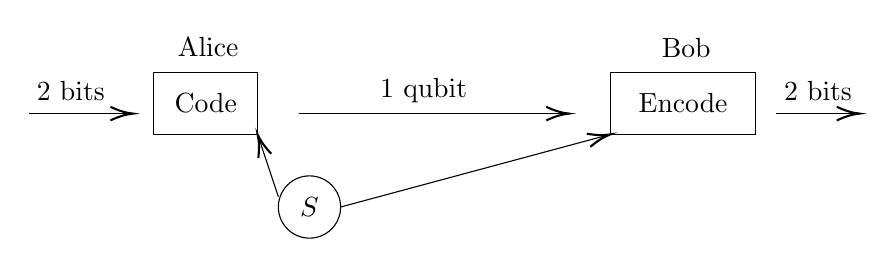
\begin{tikzpicture}[x=0.75pt,y=0.75pt,yscale=-1,xscale=1]
%uncomment if require: \path (0,300); %set diagram left start at 0, and has height of 300

%Shape: Rectangle [id:dp31062974555219114] 
\draw   (160,80) -- (210,80) -- (210,110) -- (160,110) -- cycle ;
%Shape: Rectangle [id:dp20682163383027818] 
\draw   (380,80) -- (450,80) -- (450,110) -- (380,110) -- cycle ;
%Shape: Circle [id:dp4743769670991709] 
\draw   (220,145) .. controls (220,136.72) and (226.72,130) .. (235,130) .. controls (243.28,130) and (250,136.72) .. (250,145) .. controls (250,153.28) and (243.28,160) .. (235,160) .. controls (226.72,160) and (220,153.28) .. (220,145) -- cycle ;
%Straight Lines [id:da5477596148170991] 
\draw    (220,140) -- (210.63,111.9) ;
\draw [shift={(210,110)}, rotate = 431.57] [color={rgb, 255:red, 0; green, 0; blue, 0 }  ][line width=0.75]    (10.93,-3.29) .. controls (6.95,-1.4) and (3.31,-0.3) .. (0,0) .. controls (3.31,0.3) and (6.95,1.4) .. (10.93,3.29)   ;

%Straight Lines [id:da9241704248293399] 
\draw    (250,145) -- (378.07,110.52) ;
\draw [shift={(380,110)}, rotate = 524.9300000000001] [color={rgb, 255:red, 0; green, 0; blue, 0 }  ][line width=0.75]    (10.93,-3.29) .. controls (6.95,-1.4) and (3.31,-0.3) .. (0,0) .. controls (3.31,0.3) and (6.95,1.4) .. (10.93,3.29)   ;

%Straight Lines [id:da19977175053033802] 
\draw    (100,100) -- (148,100) ;
\draw [shift={(150,100)}, rotate = 180] [color={rgb, 255:red, 0; green, 0; blue, 0 }  ][line width=0.75]    (10.93,-3.29) .. controls (6.95,-1.4) and (3.31,-0.3) .. (0,0) .. controls (3.31,0.3) and (6.95,1.4) .. (10.93,3.29)   ;

%Straight Lines [id:da30234793694339834] 
\draw    (230,100) -- (358,100) ;
\draw [shift={(360,100)}, rotate = 180] [color={rgb, 255:red, 0; green, 0; blue, 0 }  ][line width=0.75]    (10.93,-3.29) .. controls (6.95,-1.4) and (3.31,-0.3) .. (0,0) .. controls (3.31,0.3) and (6.95,1.4) .. (10.93,3.29)   ;

%Straight Lines [id:da08941647542512188] 
\draw    (460,100) -- (498,100) ;
\draw [shift={(500,100)}, rotate = 180] [color={rgb, 255:red, 0; green, 0; blue, 0 }  ][line width=0.75]    (10.93,-3.29) .. controls (6.95,-1.4) and (3.31,-0.3) .. (0,0) .. controls (3.31,0.3) and (6.95,1.4) .. (10.93,3.29)   ;


% Text Node
\draw (185,95) node  [align=left] {Code};
% Text Node
\draw (415,95) node  [align=left] {Encode};
% Text Node
\draw (235,145) node   {$S$};
% Text Node
\draw (120,89) node  [align=left] {2 bits};
% Text Node
\draw (290,89) node  [align=left] {1 qubit};
% Text Node
\draw (480,89) node  [align=left] {2 bits};
% Text Node
\draw (186.17,67.67) node  [align=left] {Alice};
% Text Node
\draw (416.5,68.33) node  [align=left] {Bob};

\end{tikzpicture}
\caption{Schema del protocollo di Dense Coding\label{fig:dense-coding}}
\end{figure}

\begin{figure}[H]
\centering
\tikzset{every picture/.style={line width=0.75pt}} %set default line width to 0.75pt        

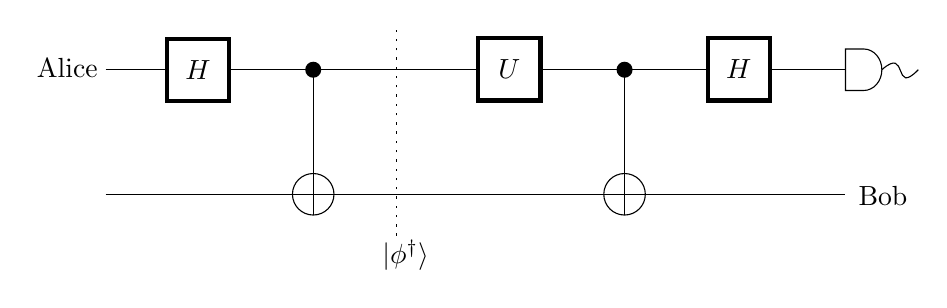
\begin{tikzpicture}[x=0.75pt,y=0.75pt,yscale=-1,xscale=1]
%uncomment if require: \path (0,300); %set diagram left start at 0, and has height of 300

%Straight Lines [id:da9095170240086292] 
\draw    (140,140) -- (230,140) ;


%Shape: Square [id:dp8070908790790741] 
\draw  [line width=1.5]  (169.5,65.2) -- (199.5,65.2) -- (199.5,95.2) -- (169.5,95.2) -- cycle ;
%Flowchart: Or [id:dp05168943682872462] 
\draw   (230,140) .. controls (230,134.48) and (234.48,130) .. (240,130) .. controls (245.52,130) and (250,134.48) .. (250,140) .. controls (250,145.52) and (245.52,150) .. (240,150) .. controls (234.48,150) and (230,145.52) .. (230,140) -- cycle ; \draw   (230,140) -- (250,140) ; \draw   (240,130) -- (240,150) ;
%Straight Lines [id:da029886615395413596] 
\draw    (240,80) -- (240,130) ;

\draw [shift={(240,80)}, rotate = 90] [color={rgb, 255:red, 0; green, 0; blue, 0 }  ][fill={rgb, 255:red, 0; green, 0; blue, 0 }  ][line width=0.75]      (0, 0) circle [x radius= 3.35, y radius= 3.35]   ;
%Straight Lines [id:da29236840670166764] 
\draw    (240,80) -- (320,80) ;


%Shape: Square [id:dp129175975552557] 
\draw  [line width=1.5]  (319.5,64.8) -- (349.5,64.8) -- (349.5,94.8) -- (319.5,94.8) -- cycle ;
%Shape: Square [id:dp10761665023417288] 
\draw  [line width=1.5]  (430,64.8) -- (460,64.8) -- (460,94.8) -- (430,94.8) -- cycle ;
%Flowchart: Or [id:dp5316772768296039] 
\draw   (380,140) .. controls (380,134.48) and (384.48,130) .. (390,130) .. controls (395.52,130) and (400,134.48) .. (400,140) .. controls (400,145.52) and (395.52,150) .. (390,150) .. controls (384.48,150) and (380,145.52) .. (380,140) -- cycle ; \draw   (380,140) -- (400,140) ; \draw   (390,130) -- (390,150) ;
%Straight Lines [id:da5621342120352391] 
\draw    (390,80) -- (390,130) ;

\draw [shift={(390,80)}, rotate = 90] [color={rgb, 255:red, 0; green, 0; blue, 0 }  ][fill={rgb, 255:red, 0; green, 0; blue, 0 }  ][line width=0.75]      (0, 0) circle [x radius= 3.35, y radius= 3.35]   ;
%Straight Lines [id:da4778886014678565] 
\draw    (350,80) -- (430,80) ;


%Straight Lines [id:da6512821890223695] 
\draw    (400,140) -- (496.43,140) ;


%Straight Lines [id:da44088069165233645] 
\draw    (250,140) -- (380,140) ;


%Straight Lines [id:da7489348301333347] 
\draw    (200,80) -- (240,80) ;


%Straight Lines [id:da8059166751569593] 
\draw    (140,80) -- (170,80) ;


%Straight Lines [id:da29091713857112866] 
\draw    (460,80) -- (496.53,80) ;


%Flowchart: Delay [id:dp4305677846822096] 
\draw   (496.43,70) -- (505.2,70) .. controls (510.04,70) and (513.97,74.48) .. (513.97,80) .. controls (513.97,85.52) and (510.04,90) .. (505.2,90) -- (496.43,90) -- cycle ;
%Curve Lines [id:da8295120860975134] 
\draw    (513.97,80) .. controls (527.12,68.33) and (518.93,93) .. (531.5,80) ;


%Straight Lines [id:da7084663542816965] 
\draw  [dash pattern={on 0.84pt off 2.51pt}]  (280,160) -- (280,60) ;



% Text Node
\draw (184.5,80.2) node   {$H$};
% Text Node
\draw (334.5,79.8) node   {$U$};
% Text Node
\draw (445,79.8) node   {$H$};
% Text Node
\draw (121.5,79) node  [align=left] {Alice};
% Text Node
\draw (514.5,141) node  [align=left] {Bob};
% Text Node
\draw (284.5,169.5) node   {$|\phi ^{\dagger } \rangle $};


\end{tikzpicture}
\caption{Rappresentazione del canale come azione di gate quantistici\label{fig:dense-coding-gates}}
\end{figure}

Il protocollo consiste nei seguenti passi:
\begin{enumerate}
\item \textbf{Preparazione}. Si crea uno stato entangled:
\begin{align*}
\ket{\phi^+} = \op{CNOT}(H\otimes \bb{I})\ket{00} = \frac{1}{\sqrt{2}}(\ket{00}+\ket{11})
\end{align*}
I due qubit vengono poi lasciati uno ad $A$ e uno a $B$.
\item \textbf{Messaggio}. Alice sceglie quali $2$ bit classici inviare, e a seconda della scelta compie una certa operazione $U$ sul suo qubit.

\begin{table}[H]
\centering
\begin{tabular}{cc}
\toprule
\textbf{Bit} & $\bm{U}$ \\ \midrule
00 & $\bb{I}$\\
01 & $\hat{\sigma}_x$\\
10 & $\hat{\sigma}_y$\\
11 & $\hat{\sigma}_z$ \\ \bottomrule
\end{tabular}
\caption{Operazioni $U$ svolte da Alice a seconda della combinazione dei $2$ bit classici che vuole inviare a Bob}
\end{table}

Avremo quindi $4$ possibili stati finali per $\ket{\phi^+}$:
\begin{align*}
(\bb{I}\otimes \bb{I}) \ket{\phi^+} &= \ket{\phi^+}\\
(\hat{\sigma}_x \otimes \bb{I}) \ket{\phi^+} &= \frac{1}{\sqrt{2}} (\ket{10}+\ket{01}) = \ket{\psi^+}\\
(\hat{\sigma_z} \otimes \bb{I}) \ket{\phi^+} &= \frac{1}{\sqrt{2}}(\ket{00}-\ket{11}) = \ket{\phi^-}\\
(\hat{\sigma}_y \otimes \bb{I}) \ket{\phi^+} &= \ket{\psi^-}
\end{align*}

\item \textbf{Comunicazione}: Alice manda il suo qubit a Bob
\item \textbf{Misura} Bob esegue l'operazione inversa di quella al punto $1$ sui due qubit che ora possiede, e il cui è stato è un certo $\ket{\psi}$:
\begin{align*}
[\op{CNOT}(H \otimes \bb{I})]^{-1} \ket{\psi} = B
\end{align*}
Calcolando il risultato nei $4$ casi vediamo come si riottengano gli stati della base computazionale, che Bob può esaminare per riottenere i $2$ bit classici scelti da Alice al punto 2:
\begin{align*}
B \ket{\phi^+} &= \ket{00}\\
B \ket{\phi^-} &= \ket{10}\\
B\ket{\psi^+} &= \ket{01}\\
B\ket{\psi^-} &= \ket{11}
\end{align*}
\end{enumerate}

\end{document}


